\section{Strategy's Capital Structure}
\label{sec:capital_structure}

Strategy has built something that resembles a synthetic collateralized debt obligation, except with a single underlying asset. Traditional CDOs derive whatever stability they have from pooling uncorrelated assets; MSTR offers only the appearance of diversification through seniority. Every tranche, from senior convertible debt to junior preferred shares to common equity, is backed by the same thing: Bitcoin. When BTC falls, everyone falls together. The seniority waterfall determines only the order in which different investors get wiped out, not whether they avoid exposure to the underlying risk.

Figure~\ref{fig:capital_structure} illustrates the hierarchy of claims as of January 2026.

\begin{figure}[H]
    \centering
    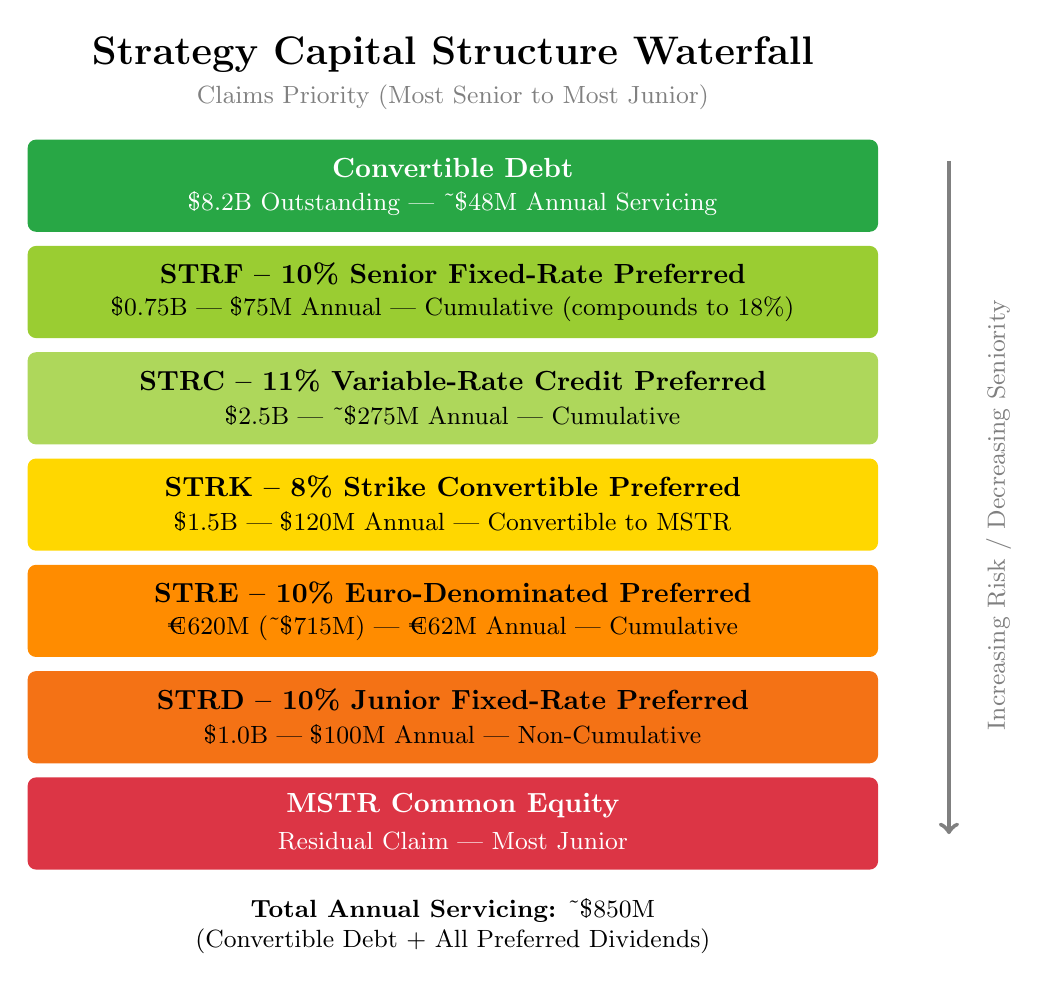
\begin{tikzpicture}[scale=0.9]
        % Define colors - green (safest) to red (riskiest)
        \definecolor{safest}{RGB}{40,167,69}
        \definecolor{seniorpref}{RGB}{154,205,50}
        \definecolor{midpref}{RGB}{255,215,0}
        \definecolor{juniorpref}{RGB}{255,140,0}
        \definecolor{riskiest}{RGB}{220,53,69}

        % Title
        \node[font=\Large\bfseries] at (6,11) {Strategy Capital Structure Waterfall};
        \node[font=\small,gray] at (6,10.4) {Claims Priority (Most Senior to Most Junior)};

        % Boxes - from top (senior/safest) to bottom (junior/riskiest)
        % 1. Convertible Debt - SAFEST (green)
        \fill[safest, rounded corners=3pt] (0,8.5) rectangle (12,9.8);
        \node[white, font=\bfseries] at (6,9.4) {Convertible Debt};
        \node[white, font=\small] at (6,8.9) {\$8.2B Outstanding | \textasciitilde\$48M Annual Servicing};

        % 2. STRF - Senior Fixed (yellow-green)
        \fill[seniorpref, rounded corners=3pt] (0,7) rectangle (12,8.3);
        \node[black, font=\bfseries] at (6,7.9) {STRF -- 10\% Senior Fixed-Rate Preferred};
        \node[black, font=\small] at (6,7.4) {\$0.75B | \$75M Annual | Cumulative (compounds to 18\%)};

        % 3. STRC - Variable (yellow-green lighter)
        \fill[seniorpref!80!white, rounded corners=3pt] (0,5.5) rectangle (12,6.8);
        \node[black, font=\bfseries] at (6,6.4) {STRC -- 11\% Variable-Rate Credit Preferred};
        \node[black, font=\small] at (6,5.9) {\$2.5B | \textasciitilde\$275M Annual | Cumulative};

        % 4. STRK - Strike (yellow)
        \fill[midpref, rounded corners=3pt] (0,4) rectangle (12,5.3);
        \node[black, font=\bfseries] at (6,4.9) {STRK -- 8\% Strike Convertible Preferred};
        \node[black, font=\small] at (6,4.4) {\$1.5B | \$120M Annual | Convertible to MSTR};

        % 5. STRE - Euro (orange)
        \fill[juniorpref, rounded corners=3pt] (0,2.5) rectangle (12,3.8);
        \node[black, font=\bfseries] at (6,3.4) {STRE -- 10\% Euro-Denominated Preferred};
        \node[black, font=\small] at (6,2.9) {\texteuro620M (\textasciitilde\$715M) | \texteuro62M Annual | Cumulative};

        % 6. STRD - Junior (orange-red)
        \fill[juniorpref!70!riskiest, rounded corners=3pt] (0,1) rectangle (12,2.3);
        \node[black, font=\bfseries] at (6,1.9) {STRD -- 10\% Junior Fixed-Rate Preferred};
        \node[black, font=\small] at (6,1.4) {\$1.0B | \$100M Annual | Non-Cumulative};

        % 7. Common Equity - RISKIEST (red)
        \fill[riskiest, rounded corners=3pt] (0,-0.5) rectangle (12,0.8);
        \node[white, font=\bfseries] at (6,0.4) {MSTR Common Equity};
        \node[white, font=\small] at (6,-0.1) {Residual Claim | Most Junior};

        % Arrow indicating seniority
        \draw[->, ultra thick, gray] (13,9.5) -- (13,0);
        \node[rotate=90, gray, font=\small] at (13.7,4.5) {Increasing Risk / Decreasing Seniority};

        % Total servicing annotation
        \node[font=\small, align=center] at (6,-1.3) {%
            \textbf{Total Annual Servicing:} \textasciitilde\$850M \\
            (Convertible Debt + All Preferred Dividends)
        };
    \end{tikzpicture}
    \caption{Strategy Capital Structure Waterfall. The figure shows the seniority hierarchy of MSTR's financing instruments, from most senior (convertible debt) to most junior (common equity). All claims are effectively backed by Bitcoin holdings. Annual servicing costs total approximately \$850 million.}
    \label{fig:capital_structure}
\end{figure}

\subsection{Convertible Debt}

The convertible notes sit atop the capital structure and represent the most senior claim. Strategy has \$8.2 billion in convertible notes outstanding with a weighted average coupon of 0.42\% and maturities staggered from 2028 to 2032. Annual cash servicing runs approximately \$48 million. The notes convert to MSTR shares at premiums to the issuance price, and in liquidation, convertible holders would be paid before anyone else.

The low-coupon structure is elegant from Strategy's perspective: it minimizes cash outflows while the embedded call option provides upside to investors who care about that sort of thing. But the primary buyers aren't playing for equity upside. Convertible arbitrage hedge funds buy these instruments for the volatility exposure. They don't care whether MSTR stock goes up or down; they care that it moves. Strategy has captured roughly 30\% of the U.S. convertible debt market in 2025 alone, reflecting insatiable arb fund demand for high-vol paper.

\subsection{Preferred Share Instruments}

Strategy has issued five distinct series of preferred shares, each designed to tap a different investor base. Table~\ref{tab:preferred_summary} summarizes the terms.

\begin{table}[H]
\centering
\caption{Summary of Strategy Preferred Share Instruments (January 2026)}
\label{tab:preferred_summary}
\begin{tabular}{@{}llrrll@{}}
\toprule
\textbf{Ticker} & \textbf{Name} & \textbf{Notional} & \textbf{Annual Cost} & \textbf{Rate} & \textbf{Cumulative?} \\
\midrule
STRF & Strife & \$0.75B & \$75M & 10\% fixed & Yes (to 18\%) \\
STRC & Stretch & \$2.50B & \$275M & 11\% variable & Yes \\
STRK & Strike & \$1.50B & \$120M & 8\% fixed & Yes \\
STRE & Stream & \$0.72B & \$72M & 10\% fixed & Yes \\
STRD & Stride & \$1.00B & \$100M & 10\% fixed & No \\
\midrule
\multicolumn{2}{l}{\textbf{Total Preferred}} & \textbf{\$6.47B} & \textbf{\$642M} & & \\
\bottomrule
\end{tabular}
\end{table}

Note: These figures represent current outstanding amounts, which continue to grow as Strategy executes its ``42/42'' capital plan targeting \$84 billion in total issuance by 2027. VanEck projects preferred equity reaching \$15.5 billion by end of 2026.

Why preferreds rather than more debt? Several reasons. Preferred shares don't count as debt for leverage ratios and covenants, preserving whatever financial flexibility Strategy claims to have. They're perpetual, eliminating refinancing risk (though creating a permanent servicing burden). Missing a preferred dividend doesn't trigger default the way missing bond interest would, though cumulative preferreds accrue unpaid dividends that eventually come due. And preferreds sit between debt and equity in the capital structure, avoiding the immediate dilution of ATM equity offerings while still accessing capital.

The different series target different appetites. STRF offers 10\% fixed with cumulative compounding to 18\% if dividends are missed (a punishing feature that incentivizes payment). STRC floats with rates (currently 11\%) and appeals to investors worried about duration risk. STRK converts to common equity at \$1,000 per MSTR share, providing upside exposure. STRE taps European investors through the Luxembourg Euro MTF exchange. STRD, the junior tranche, offers 10\% but non-cumulative dividends: if Strategy misses a payment, STRD holders have no legal claim to catch up.

\subsection{Seniority Analysis}

In distress, claims get paid in order: convertible debt first, then STRF, then STRC, then STRK, then STRE, then STRD, and finally common equity if anything remains. This waterfall creates synthetic subordination. The preferred layers provide a cushion that improves the credit quality of senior instruments, at the cost of concentrating risk in the junior tranches.

Common equity holders bear first losses. This isn't a bug; it's the design. MSTR equity behaves like a leveraged call option on Bitcoin, with the aggregate claims of senior instruments serving as the strike price. In a rising BTC environment, equity captures amplified upside. In a declining environment, equity absorbs amplified losses until it's wiped out, at which point the pain starts moving up the capital structure.

\subsection{The USD Reserve}

Strategy maintains a dedicated USD reserve for preferred dividend payments and debt service. As of January 4, 2026, this reserve stood at \$2.25 billion, a substantial improvement from the minimal cash buffers of earlier years. At current servicing costs of approximately \$850 million annually, the reserve provides roughly 32 months of coverage assuming no additional cash generation.

This buffer transforms the company's liquidity position. The legacy enterprise analytics business continues to generate \$40-50 million in annual operating cash flow, providing ongoing liquidity independent of capital markets. Combined with the USD reserve, Strategy could survive an extended period of capital market closure without selling Bitcoin.

The arithmetic: \$2.25B reserve plus roughly \$90M operating cash flow over 32 months yields approximately \$2.34 billion in available liquidity. Against \$2.27 billion in servicing costs over the same period (\$850M $\times$ 2.67 years), the buffer is adequate. This represents a significant de-risking compared to earlier periods when the company operated with minimal cash.

However, each new preferred issuance increases the servicing burden. VanEck projects annual preferred dividends rising from \$642 million currently to over \$900 million by end of 2026 as the 42/42 plan progresses. The reserve must grow proportionally to maintain the same coverage ratio.

\subsection{Implications}

The capital structure reveals several dynamics relevant to the rest of this analysis. Strategy has constructed a synthetic credit hierarchy where every tranche bears the same underlying Bitcoin risk; seniority determines loss allocation, not loss avoidance. The \$850 million annual servicing cost (growing toward \$1 billion) creates a breakeven requirement that constrains the scenario analysis in Section~\ref{sec:results}. Common equity holders are effectively long a leveraged call option on Bitcoin, with senior claims acting as the strike. And the Merton model in Section~\ref{sec:methodology} can formalize this option-like payoff structure mathematically.
